\documentclass{article}
\usepackage[citecolor=bleu]{hyperref}
\usepackage{amsmath,amsthm,amssymb}
\newtheorem{lemma}{Lemma}
\usepackage{xcolor}
\input{../slides/notations}
\usepackage[natbib=true,backend=biber,citestyle=authoryear]{biblatex}
\bibliography{../bib/stats,../bib/learning}

\usepackage{tikz}
\usetikzlibrary{bayesnet}
\usetikzlibrary{arrows}


\title{BML: exercise sheet}
\date{}

\begin{document}
\maketitle

Stars indicate the difficulty level, from 1 to 3. One star means that everyone should be able to do it without too much effort.

\section{Lecture \#1: Bayesics}

\subsection{Conjugate priors 101: Gaussians $(\star)$}
\label{s:gaussianConjugacy}
Let $y\vert\mu \sim \cN(\mu,I_N)$ and $\mu\sim \cN(0,a I_N)$, for some $a>0$. Show that
\begin{equation}
  \mu\vert y \sim \cN(b y,bI_N), \text{ where } b=a/(a+1).
  \label{e:gaussianConjugacy}
\end{equation}

\subsection{A conjugate prior on probability vectors $(\star)$}
Let
$$
\Delta_d = \{\theta\in\mathbb[0,1]^d \text{ such that } \sum_{k=1}^d \theta_d = 1\}.
$$
Let further $\alpha\in(\mathbb{R}_+)^d$. The Dirichlet pdf is defined by
 $$
 \text{Dir}(\theta\vert \alpha) = \frac{1}{B(\alpha)} \prod_{k=1}^d \theta_k^{\alpha_k -1} 1_{\theta\in \Delta_d},$$
where
 $ B(\alpha) = \prod_{k=1}^d \Gamma(\alpha_k) / \Gamma(\sum_{k=1}^d \alpha_k)$
 is the so-called beta function.

 Now put a prior $\text{Dir}(\theta\vert \alpha)$ on $\theta$, and consider drawing $y_{1:N}$ from the multinomial distribution with parameter $\theta\in\Delta_d$. Show that
 \begin{equation}
   p(\theta, y_{1:N}) = \frac{B(\alpha+c)}{B(\alpha)} \text{Dir}(\theta\vert \alpha),
\label{e:joint}
 \end{equation}
 where $c=(\sum_{i=1}^N 1_{y_i=k})_{1\leq k \leq d}$ is the vector of counts. Note that \eqref{e:joint} implies that $\theta\vert y_{1:N} \sim \text{Dir}(\theta\vert \alpha)$ and that the marginal likelihood $p(y_{1:n}) = B(\alpha)/B(\alpha+c)$.

 \subsection{Estimating the mean of a Gaussian $(\star\star)$}
 Let $\mu =(\mu_1,\dots,\mu_N)\in \mathbb{R}^N$, and consider $N$ i.i.d. real variables $y_i\vert \mu \sim \cN(\mu_i, 1)$. We wish to infer $\mu$.
\begin{enumerate}
\item What is the maximum likelihood estimator $\hat\mu_{\text{MLE}}$?
\item Henceforth, we judge estimators by the square loss. The frequentist risk of an estimator $\hat\mu$ is
 $$ R(\hat\mu) = \mathbb{E}_{y\vert\mu}  \Vert \mu - \hat\mu\Vert^2.$$
 show that $R(\hat\mu_{\text{MLE}}) = N$.
\item Suppose we have prior belief that $\mu$ lies near $0$, and we choose to represent it by $\mu\sim \cN(0,aI_N),$ $a>0$. What is the Bayes estimator $\hat\mu_{\text{Bayes}}$? What is its (frequentist) risk $R(\hat\mu_{\text{Bayes}})$? What is its Bayes risk $\mathbb{E}_\mu R(\hat\mu_{\text{Bayes}})$?
\item Since we actually have no idea what $a$ should be, we propose to estimate it from data\footnote{This procedure of using data to tune the prior is called \emph{empirical Bayes} (EB). The expected utility principle allows it, but statisticians who like to interpret their prior as encoding their belief before the data is collected are uncomfortable with EB. At the other extreme, Bayesians who insist on using estimators with good frequentist properties are happy using the data or the likelihood to design their prior.} Show that the marginal of $y$ is
$$
\int p(y,\mu)\d \mu = \cN (y\vert 0,(a+1)I_N).
$$
In particular, what is the law of $S= \Vert y\Vert^2$? Deduce from it that $(N-2)/S$ is an unbiased estimator of $a+1$, and consider the empirical Bayes estimator $$\hat\mu_\text{EB} = \left(1- \frac{N-2}{S}\right)y.$$
What is its Bayes risk?
\item \emph{Note: This particular item is $(\star\star\star)$ because it is longer to solve, but all individual arguments are elementary; do this only if you have solved all the preceding exercises, though. Also, see \cite[Section 1.2]{Efr10} for a solution)} Show that for $N\geq 3$, for every $\mu\in\mathbb{R}^N$,
\begin{equation}
R(\hat\mu_\text{EB}) < R(\hat\mu_\text{MLE}).
\label{e:stein}
\end{equation}
Frequentists say that $\hat\mu_\text{EB}$ dominates $\mu_\text{MLE}$, in the sense that whatever the value of $\mu$, the risk of $\hat\mu_\text{EB}$ is the smallest of the two. This happens even when $\mu$ is far from zero, in which case one might have thought that our $\cN(0,aI_N)$ prior would have been a poor choice. Finally, if you are a strict Waldian, you should thus prefer $\hat\mu_\text{EB}$ to $\hat\mu_\text{MLE}$. Many applied frequentists still use $\hat\mu_\text{MLE}$, however; see \citep[Section 1.3]{Efr10} for a tentative answer.

Equation~\ref{e:stein} is called the James-Stein effect, and is a standard example of why following Bayesian guidelines can end up giving good frequentist estimators. Shrinkage, like $\hat\mu_\text{EB}$ shrinks $\hat\mu_\text{MLE}$ towards zero, is now commonplace in large-dimensional regression. For more on frequentist guarantees for Bayesian estimators and shrinkage, see \citep[Sections 7, 8, 9]{PaIn09}.
\end{enumerate}

\subsection{Classification with asymmetric loss ($\star$)}
Consider the classification problem, but with loss
$$
L(a_g,s) = \alpha 1_{y\neq g(x; x_{1:n}, y_{1:n})} 1_{y=0} + \beta 1_{y\neq g(x; x_{1:n}, y_{1:n})} 1_{y=1},
$$
for some $\alpha,\beta>0$.
Show that the Bayes decision rule is
$$ g^\star(x; x_{1:n}, y_{1:n}) = 1_{p(y\vert x, x_{1:n}, y_{1:n}) \geq \frac{\alpha}{\alpha+\beta}}.$$
In particular, if $\alpha\ll\beta$, one will often decide for predicting $1$, because the cost for misclassifying a 0 is low.
\subsection{Linear regression with a Gaussian prior $(\star)$}
It is all in the title: show that the posterior is Gaussian, with mean the ridge regression estimator.

 \subsection{For more exercises on Bayesian derivations}
 \begin{itemize}
   \item Exercises 5.1 to 5.4 of \citep{Mur12}.
   \item Go through Sections 4.4 to 4.6 of \citep{Mur12} with pen and paper. Linear Gaussian models appear all the time.
   \item Exercises 2.6, 2.9, 2.10, 2.13, 2.14, and 2.15 of \citep{MaRo07}. Solutions are \href{https://arxiv.org/abs/0910.4696}{here}.
 \end{itemize}

\section{Lecture \#2: MCMC}

\subsection{DAGs and dependence ($\star$)}
\begin{figure}
  \centering
  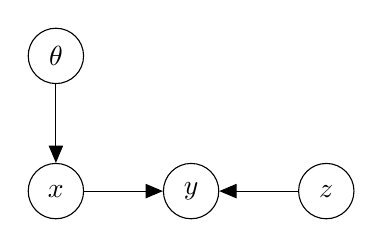
\begin{tikzpicture}
  \node[latent] (y) {$y$};
  \node[latent,right= of y] (z) {$z$}; %
  \node[latent,left= of y] (x) {$x$}; %
  \node[latent,above= of x] (t) {$\theta$}; %
  \edge x y;
  \edge z y;
  \edge t x;
\end{tikzpicture}
\caption{A DAG}
\label{f:dag}
\end{figure}

Consider the DAG from Figure~\ref{f:dag}.
\begin{enumerate}
\item Write the corresponding factorization of $p(x,y,z,\theta)$.
\item Deduce from the factorization that $x\perp z$.
\item\label{i:markov} Deduce from the factorization that $x\perp z\vert\theta$.
\item\label{i:away} Deduce from the factorization that $x\not\perp z\vert \theta, y$.
\end{enumerate}
In particular, note how Item~\ref{i:markov} is a case of \emph{being independent from your non-descendents given your parents}, while Item~\ref{i:away} illustrates how conditioning on common children can induce dependence between parents. In more complicated DAGs, the so-called \emph{Bayes ball} algorithm determines whether two sets of nodes are independent given a third one; see \cite[Section 10.5]{Mur12}.

\subsection{Self-normalized importance sampling ($\star\star$)}
Show a central limit theorem for the self-normalized importance sampling estimator. Hint: use the delta method.

\subsection{Systematic scan Gibbs sampler ($\star\star$)}
Show that the systematic scan Gibbs kernel, while not satisfying detailed balance, leaves $\pi$ invariant.

\subsection{Gibbs ($\star$) and collapsed ($\star\star$) Gibbs for LDA}
Rederive all conditionals in the LDA and collapsed LDA model. Hint: use \eqref{e:joint}. \emph{Hint: Check \citep[Section 27.3.4]{Mur12}}.
%\subsection{Hierarchical linear regression}

\section{Lecture \#3}

\subsection{A useful lemma for variational LDA ($\star$)}
Let $\Psi(\cdot) := \Gamma'(\cdot)/\Gamma(\cdot)$ be the digamma function. Show that
$$
\mathbb{E}_{\text{Dir}(\theta\vert\alpha)} \log \theta_i = \Psi(\theta_i) - \Psi(\Vert \theta\Vert_1).
$$
We used that lemma when deriving the coordinatewise updates for VB with mean field approximation.

\subsection{VB for LDA with counts ($\star\star$)}
Derive the coordinatewise updates for VB on the count version of LDA. The variational approximation should read
$$
q(\pi_i, c_i, B) = \text{Dir}(\pi_i\vert\tilde\pi_i) \prod_v \text{Multinomial}(c_{iv\cdot}\vert n_{iv}, \tilde{c}_{iv\cdot}) \prod_k \text{Dir}(b_{\cdot k}\vert\tilde b_{\cdot k}).
$$
\emph{Hint: See \cite[Section 27.3.6]{Mur12}.}

\section{Lecture \#4}

\printbibliography

\end{document}
